\documentclass[10pt]{standalone}
\usepackage[utf8]{inputenc}
\usepackage{pgf,tikz}
\usetikzlibrary{arrows}
\usetikzlibrary{arrows.meta}
\pagestyle{empty}
\begin{document}
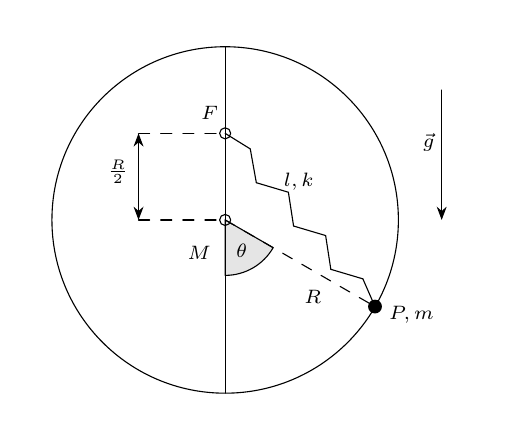
\begin{tikzpicture}[line cap=round,line join=round,>=Stealth,x=1.1cm,y=1.1cm]
\clip(-2.28,-2.29) rectangle (2.98,2.22);
\draw [shift={(0,0)},fill=black,fill opacity=0.1] (0,0) -- (-90:0.64) arc (-90:-29.98:0.64) -- cycle;
\draw(0,0) circle (2.2cm);
\draw (0,2)-- (0,-2);
\draw [dash pattern=on 4pt off 4pt] (0,0)-- (1.73,-1);
\draw [dash pattern=on 4pt off 4pt] (-1,1)-- (0,1);
\draw [dash pattern=on 4pt off 4pt] (-1,0)-- (0,0);
\draw [->] (-1,0.5) -- (-1,1);
\draw [->] (-1,0.5) -- (-1,0);
\draw (0,1)-- (0.29,0.82);
\draw (0.29,0.82)-- (0.36,0.43);
\draw (0.36,0.43)-- (0.73,0.32);
\draw (0.73,0.32)-- (0.79,-0.07);
\draw (0.79,-0.07)-- (1.16,-0.18);
\draw (1.16,-0.18)-- (1.22,-0.57);
\draw (1.22,-0.57)-- (1.59,-0.68);
\draw (1.59,-0.68)-- (1.73,-1);
\draw [->] (2.5,1.5) -- (2.5,0);
\begin{scriptsize}
\draw [color=black] (0,0) circle (2.0pt);
\draw[color=black] (-0.3,-0.38) node {$M$};
\draw [color=black] (0,1) circle (2.0pt);
\draw[color=black] (-0.18,1.24) node {$F$};
\fill [color=black] (1.73,-1) circle (2.5pt);
\draw[color=black] (2.15,-1.09) node {$P,m$};
\draw[color=black] (1.01,-0.89) node {$R$};
\draw[color=black] (0.19,-0.36) node {$\theta$};
\draw[color=black] (-1.24,0.56) node {$\frac{R}{2}$};
\draw[color=black] (0.85,0.44) node {$l,k$};
\draw[color=black] (2.35,0.89) node {$\vec{g}$};
\end{scriptsize}
\end{tikzpicture}
\end{document}